%==============================================================================
% Sjabloon onderzoeksvoorstel bachelorproef
%==============================================================================
% Gebaseerd op LaTeX-sjabloon ‘Stylish Article’ (zie voorstel.cls)
% Auteur: Jens Buysse, Bert Van Vreckem
%
% Compileren in TeXstudio:
%
% - Zorg dat Biber de bibliografie compileert (en niet Biblatex)
%   Options > Configure > Build > Default Bibliography Tool: "txs:///biber"
% - F5 om te compileren en het resultaat te bekijken.
% - Als de bibliografie niet zichtbaar is, probeer dan F5 - F8 - F5
%   Met F8 compileer je de bibliografie apart.
%
% Als je JabRef gebruikt voor het bijhouden van de bibliografie, zorg dan
% dat je in ``biblatex''-modus opslaat: File > Switch to BibLaTeX mode.

\documentclass{voorstel}

\usepackage{lipsum}

%------------------------------------------------------------------------------
% Metadata over het voorstel
%------------------------------------------------------------------------------

%---------- Titel & auteur ----------------------------------------------------

% TODO: geef werktitel van je eigen voorstel op
\PaperTitle{Veiligheidsproblemen in container orchestration tools: Wat zijn en hoe kunnen we ze vermijden? }
\PaperType{Onderzoeksvoorstel Bachelorproef 2020-2021} % Type document

% TODO: vul je eigen naam in als auteur, geef ook je emailadres mee!
\Authors{Nick Heymans\textsuperscript{1}} % Authors
\CoPromotor{?????????\textsuperscript{2} (Bedrijfsnaam)}
\affiliation{\textbf{Contact:}
  \textsuperscript{1} \href{mailto:nick.heymans@student.hogent.be}{nick.heymans@student.hogent.be};
  \textsuperscript{2} \href{mailto:piet.pieters@acme.be}{piet.pieters@acme.be};
}

%---------- Abstract ----------------------------------------------------------

\Abstract{Hier schrijf je de samenvatting van je voorstel, als een doorlopende tekst van één paragraaf. Wat hier zeker in moet vermeld worden: \textbf{Context} (Waarom is dit werk belangrijk?); \textbf{Nood} (Waarom moet dit onderzocht worden?); \textbf{Taak} (Wat ga je (ongeveer) doen?); \textbf{Object} (Wat staat in dit document geschreven?); \textbf{Resultaat} (Wat verwacht je van je onderzoek?); \textbf{Conclusie} (Wat verwacht je van van de conclusies?); \textbf{Perspectief} (Wat zegt de toekomst voor dit werk?).

Bij de sleutelwoorden geef je het onderzoeksdomein, samen met andere sleutelwoorden die je werk beschrijven.

Vergeet ook niet je co-promotor op te geven.
}

%---------- Onderzoeksdomein en sleutelwoorden --------------------------------
% TODO: Sleutelwoorden:
%
% Het eerste sleutelwoord beschrijft het onderzoeksdomein. Je kan kiezen uit
% deze lijst:
%
% - Mobiele applicatieontwikkeling
% - Webapplicatieontwikkeling
% - Applicatieontwikkeling (andere)
% - Systeembeheer
% - Netwerkbeheer
% - Mainframe
% - E-business
% - Databanken en big data
% - Machineleertechnieken en kunstmatige intelligentie
% - Andere (specifieer)
%
% De andere sleutelwoorden zijn vrij te kiezen

\Keywords{Onderzoeksdomein. Containerization --- Security --- Container Orchestration } % Keywords
\newcommand{\keywordname}{Sleutelwoorden} % Defines the keywords heading name

%---------- Titel, inhoud -----------------------------------------------------

\begin{document}

\flushbottom % Makes all text pages the same height
\maketitle % Print the title and abstract box
\tableofcontents % Print the contents section
\thispagestyle{empty} % Removes page numbering from the first page

%------------------------------------------------------------------------------
% Hoofdtekst
%------------------------------------------------------------------------------

% De hoofdtekst van het voorstel zit in een apart bestand, zodat het makkelijk
% kan opgenomen worden in de bijlagen van de bachelorproef zelf.
%---------- Inleiding en State-of-the-art ---------------------------------------------------------

\section{Inleiding en State-of-the-art} % The \section*{} command stops section numbering
\label{sec:Inleiding en State-of-the-art}

\subsection{Wat zijn containers?}
Het uitrollen en schalen van applicaties wordt steeds vaker gedaan met behulp van containers. 
Tijdens de ontwikkeling van traditionele applicaties wordt de applicatie ontwikkeld in een specifiek testomgeving. 
Vervolgens wordt de applicatie overgezet naar de productieomgeving wat vaak voor problemen zorgt (bijvoorbeeld van een linux testomgeving naar een Windows productieomgeving). 
Een container is een pakket waar één enkele applicatie in zit, samen met alle nodige afhankelijkheden\autocite{Education2019}. 
Dit zorgt ervoor dat deze gemakkelijk en snel van de ene omgeving naar de andere kan overgezet worden. 
De containers maken gebruik van een 'runtime engine', dit is een laag die verantwoordelijk is voor de communicatie tussen het operating system van de host machine en de containers zelf. 
De meeste gebruikte 'runtime engine' is de 'Docker Engine'\footnote{https://docs.docker.com/engine/}. Deze is al sinds 2013 de industriestandaard als het gaat over container software\autocite{McCarty2018}. 
Naarmate het gebruik van containers steeg, steeg ook de nood naar op manier om deze vanuit één centrale locatie te beheren. 
Om aan deze vraag te voldoen werden container orkestratie tools, zoals Kubernetes \footnote{https://kubernetes.io/}, ontwikkeld. 
Deze tools helpen bij het opzetten, uitbreiden en verbinden van een grote hoeveelheid containers. 

\subsection{Waarom container applicaties?}
Container applicaties hebben enkele voordelen tegenover normale applicaties, ze draaien namelijk geïsoleerd van de rest van het systeem. 
Ze kunnen dus perfect werken zonder afhankelijk te zijn van andere containers. 
Dit garandeerd dat als er één container aangetast is, de rest zonder interruptie kan verderwerken. 
De containers delen wel verschillende resources van het host systeem, wat de deur opent voor veiligheidsinbreuken tussen containers. 

\subsection{Context voor dit onderzoek}
Gartner \autocite{Gartner2019} voorspeld dat tegen 2022 maar liefst 75\% van alle internationale organisaties gecontaineriseerde
applicaties zullen gebruiken in hun productieomgeving. Dit zowel in lokale datacenters alsook in online cloud omgevingen. 
Uit een raport van \textcite{Tripwire2019} blijkt dat 94\% van bevraagden bezorgd zijn over de veiligheid van hun containers. 
Uit hetzelfde raport blijkt ook dat 47\% weet dat ze kwetsbare containers gebruiken in hun productieomgeving. 
Spijtig genoeg werd bij voorgaande onderzoeken, zoals \textcite{StackRox2020}, het effect van 'security best practices en tools' 
op opzetsnelheid, benodigde resources en stabiliteit steeds onderbelicht. 

\subsection{Verloop van het onderzoek}
In deze paper zal ik onderzoeken wat de belangrijkste bronnen van veiligheidsinbreuken zijn en hoe deze vermeden kunnen worden. 
Tegelijkertijd krijg ik via dit onderzoek de opportuniteit om er achter te komen of er vooral technische problemen of menselijke fouten aan de basis liggen van de veiligheidsrisico's. 
In de volgende paragraaf staat er beschreven hoe ik te werk zal gaan. 

%---------- Methodologie ------------------------------------------------------
\section{Methodologie}
\label{sec:methodologie}

Voor dit onderzoek zullen er drie scenario's opgezet worden. Elk scenario zal verschillende keren worden uitgevoerd en voor elk criteria zal het genomen worden (eventueel reking houdende met uitschieters). 
Bij elke scenario zullen er verschillende 'security best practices en tools' gebruikt worden. 
Deze zullen getest worden op basis van de volgende criteria: \newline
\begin{itemize}
	\item Deployment snelheid
	\item Benodigde resources
	\item Stabiliteit \newline
\end{itemize} 
Voorbeelden van scenario's: \newline
\begin{itemize}
	\item S(0): Er wordt een container applicatie opgezet in een Kubernetes cluster zonder extra security configuratie.
	\item S(1): Er wordt een container applicatie opgezet in een Kubernetes cluster en enkele 'best practices' worden toegepast.
	\item S(2): Er wordt een container applicatie opgezet in een Kubernetes cluster waar er gebruik word gemaakt van enkele 'security tools' zoals 'Project Calico' en 'Kube-hunter'. \newline
\end{itemize} 
Door gebruik te maken van deze scenario's en criteria hopen we vast te stellen dat het toepassen van 'security best practices en tools' een positieve invloed heeft op het gebruik van containers en orkestratie tools. 

%---------- Verwachte resultaten ----------------------------------------------
\section{Verwachte resultaten}
\label{sec:verwachte_resultaten}

Op basis van de criteria wordt er verwacht dat Scenario 0 en 1 even snel op opgezet kunnen worden en evenveel resources gebruiken. 
Ze zullen beide kwetsbaarder zijn aangezien de 'best practices' vooral bestaan uit het correct gebruik van wachtwoorden en gebruiker privileges. 
Scenario 2 daarintegen zal iets meer tijd nodig hebben om opgezet te worden(zie Figuur1) en zal daarbij meer resources gebruiken(zie Figuur2). Dit zou te wijten zijn aan de gebruikte 'security tools' die extra tijd en resource nodig hebben. 

%---------- Verwachte conclusies ----------------------------------------------
\section{Verwachte conclusies}
\label{sec:verwachte_conclusies}

Uit dit onderzoek willen we concluderen dat het toepassen van 'best practices' en het correct gebruik van security tools een positief effect teweeg brengt bij het gebruik van container orkestratie tools. 
We trachten daarnaast ook aan te duiden dat het omzeilen van security risico's een belangrijk aspect is bij het ontwikkelen van container applicaties. 
Tot slot kan er geconcludeerd worden dat het beveiligen van container clusters steeds belangrijker wordt. 
Daarnaast is het tevens van belang dat de persoon die een cluster opzet daarbij de onderliggende werkwijze goed kent en zich bewust is van de mogelijke valkuilen. 

%---------- Bijlagen ----------------------------------------------
\section{Bijlagen}
\label{sec:Bijlagen}
\begin{figure}[ht]
	\centering
	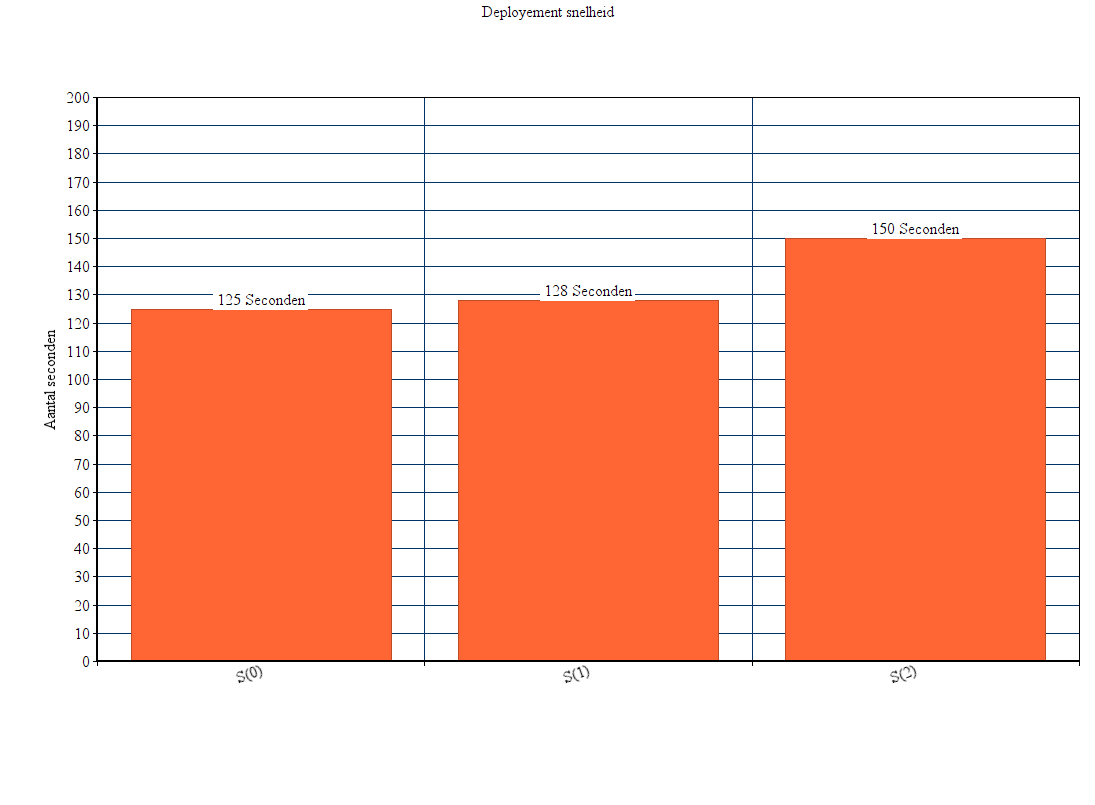
\includegraphics[width=\linewidth]{img/Mock1.png}
	\caption{Verwachte opstart tijd}
	\label{fig:example}
	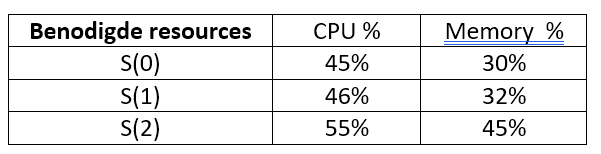
\includegraphics[width=\linewidth]{img/Mock2.png}
	\caption{Verwacht resource gebruik}
  \label{fig:example}
\end{figure}

%------------------------------------------------------------------------------
% Referentielijst
%------------------------------------------------------------------------------
% TODO: de gerefereerde werken moeten in BibTeX-bestand ``voorstel.bib''
% voorkomen. Gebruik JabRef om je bibliografie bij te houden en vergeet niet
% om compatibiliteit met Biber/BibLaTeX aan te zetten (File > Switch to
% BibLaTeX mode)

\phantomsection
\printbibliography[heading=bibintoc]

\end{document}
